\documentclass[10pt,conference]{article}
% GHI CHU: dung XeLaTeX (khong phai pdflatex) de bien dich file nay --
% dung fontspec + DejaVu Serif de ho tro day du dau tieng Viet, tranh
% han che cua goi T5/fontenc trong ban TeXLive toi gian (xem main.tex
% ban tieng Anh de biet chi tiet van de da gap phai truoc do).
% Lenh bien dich: xelatex main_vi.tex

\usepackage{fontspec}
\setmainfont{DejaVu Serif}
\usepackage{amsmath,amssymb}
\usepackage{graphicx}
\usepackage{booktabs}
\usepackage{hyperref}
\usepackage[numbers]{natbib}
\usepackage{xcolor}

\newcommand{\todo}[1]{\textcolor{red}{\textbf{[VIỆC CẦN LÀM: #1]}}}

\title{Đo lường và Cải thiện Tính Giống-Người của Lời giải CFOP do AI
Sinh ra cho Rubik's Cube: Phương pháp Trigger-Biased Search}

\author{
  Phạm Đăng Khuê \\
  Khoa Công nghệ Thông tin, Trường Đại học Điện lực\\
  pdkhue2004@gmail.com
}

\date{}

\begin{document}
\maketitle

% ============================================================
\begin{abstract}
Các phương pháp tính toán hiện có để giải Rubik's Cube — bao gồm tìm
kiếm bằng pattern-database \citep{korf1997}, các solver tối ưu dựa trên
lý thuyết nhóm \citep{rokicki2014,kociemba}, và học tăng cường
\citep{mcaleer2018} — hầu như chỉ tối ưu hóa số nước đi, tạo ra các lời
giải đúng nhưng phần lớn không thể diễn giải được đối với người học.
Ngược lại, phương pháp CFOP do con người thiết kế (Cross, F2L, OLL,
PLL) đánh đổi tính tối ưu về số nước để lấy \emph{khả năng học được},
được cấu trúc quanh một tập hữu hạn các pattern chuỗi-nước-đi dễ nhớ
("thuật toán"). Chúng tôi hình thức hóa khái niệm \emph{tính giống
người} của một kế hoạch giải cube bằng ngôn ngữ của lập kế hoạch AI
nhận biết con người (human-aware AI planning)
\citep{kulkarni2016,chakraborti2019}, đề xuất một \emph{Chỉ số
Giống-Người} (Human-Likeness Index — HLI) tổng hợp từ ba thành phần đo
lường được (khả năng phân đoạn giai đoạn, độ khớp mẫu-thuật-toán-có-tên,
và độ trùng lặp finger-trick), và giới thiệu \emph{Trigger-Biased A*
Search}, một cải tiến heuristic-search thưởng rõ ràng cho các nhánh tìm
kiếm trùng khớp với kho finger-trick của con người. Các thí nghiệm thực
nghiệm (N=60 scramble random-state cho so sánh cơ sở, đã kiểm tra độ
vững trên N=100 scramble random-move, N=60 cho quét Pareto) cho thấy
việc thiên vị heuristic tìm kiếm F2L làm tăng độ trùng lặp trigger từ mức cơ
sở 9,0\% lên 25,5\% tại $\lambda=1,0$ (Wilcoxon $p=8,3\times10^{-8}$),
với chi phí chỉ 7,4\% số nước tăng thêm (Wilcoxon $p=0,0014$), cho thấy
một sự đánh đổi Pareto thuận lợi (dù phi tuyến về thời gian tính toán).
Một nghiên cứu giám khảo con người mù, kiểu BotPrize
\citep{hingston2009} (24 mẫu, 28 người chấm) xác nhận construct
validity của HLI (Spearman $\rho=0,487$, $p=0,016$ so với điểm đánh giá
giống-người trung bình) và cho thấy Trigger-Biased Search đưa các lời
giải do AI sinh ra từ trạng thái \emph{phân biệt được về mặt thống kê
với người thật} ($p=0,005$) sang \emph{không phân biệt được về mặt
thống kê với người thật} ($p=0,109$) trong đánh giá mù. Theo hiểu biết
của chúng tôi, đây là nghiên cứu đầu tiên áp dụng các chỉ số kiểu
explicability vào một miền tìm kiếm tổ hợp quy mô lớn, kết nối AI tìm
kiếm heuristic cổ điển với nghiên cứu AI nhận biết con người và AI tác
nhân đáng tin (believable-agent AI).
\end{abstract}

% ============================================================
\section{Giới thiệu}
\label{sec:intro}

Giải Rubik's Cube từ lâu đã là một miền benchmark cho tìm kiếm
heuristic và tối ưu hóa tổ hợp \citep{korf1997,rokicki2014}, và gần đây
hơn là cho học tăng cường tự chơi (self-play reinforcement learning)
\citep{mcaleer2018}. Các phương pháp này có chung một mục tiêu: tối
thiểu hóa số nước đi (hoặc tối đa hóa tỷ lệ thắng trước một bộ sinh
scramble đối kháng), không quan tâm liệu lời giải thu được có tương ứng
với bất kỳ pattern nào mà con người có thể học, ghi nhớ, hoặc giải
thích hay không.

Ngược lại, các speedcuber con người sử dụng các phương pháp có cấu trúc
như CFOP (Cross, F2L, OLL, PLL), chủ động đánh đổi tính tối ưu về số
nước để lấy \emph{khả năng học được}: mỗi giai đoạn được rút gọn thành
việc nhận diện một trong số hữu hạn các "case" chuẩn, mỗi case đi kèm
một thuật toán cố định, có tên. Phương pháp CFOP đầy đủ gồm 57 case OLL
có tên và 21 case PLL có tên; một biến thể rút gọn được dùng rộng rãi
("2-look OLL/PLL") giải mỗi giai đoạn qua hai lượt tuần tự dùng một tập
con nhỏ hơn nhiều các thuật toán, với cái giá là tốn thêm nước đi. Hệ
thống của chúng tôi cài đặt một bảng đã kiểm chứng đầy đủ 21 case PLL
(Mục~\ref{sec:hli-conformity}). Tại thời điểm các thí nghiệm báo cáo
trong bài này được chạy, OLL chỉ có bảng 2-look (2 thuật toán sinh,
Sune/Anti-Sune, thay vì đầy đủ 57 case); sự bất đối xứng này tự nó có
giá trị thông tin cho việc đo lường Pattern-conformity
(Mục~\ref{sec:method}). Solver sau đó đã được mở rộng thành một bảng
1-look với đầy đủ 57/57 công thức đã kiểm chứng về mặt chức năng (mỗi
công thức được xác nhận không phá vỡ Cross+F2L khi áp từ trạng thái đã
giải, qua \texttt{verify\_and\_build\_table()}); trong số đó, 40/57
đã được đối chiếu đúng số thứ tự chuẩn cộng đồng (tăng dần qua nhiều
lần rà soát), số còn lại (17 công thức) hợp lệ về chức năng nhưng
chưa được đối chiếu số cộng đồng cụ thể. Riêng OLL~2 và OLL~20: toàn
bộ công thức thuần (chỉ xoay mặt đơn, không dùng nước lát/rộng) được
cộng đồng speedcubing công bố cho 2 case này đều dùng nước lát/rộng
(M/S/E hoặc r/l/f/u/d/b) --- đây là một \emph{quan sát thực nghiệm}
từ các nguồn công khai, \textbf{không phải} một chứng minh hình thức
bằng tìm kiếm vét cạn (không có script như vậy trong repo này); do đó
2 case này vẫn rơi về bảng 2-look đã kiểm chứng nói trên. Nâng cấp
bảng OLL này diễn ra sau khi thu thập dữ liệu và không làm thay đổi
các kết quả báo cáo ở Mục~\ref{sec:results}, vốn phản ánh bảng OLL 2
thuật toán sinh (Sune/Anti-Sune) có hiệu lực tại thời điểm đó.

Ba hướng nghiên cứu liên quan (Mục~\ref{sec:related}) hiện chưa giao
nhau: các solver Rubik's Cube tối ưu máy tính
(Mục~\ref{sec:related-optimal}) bỏ qua hoàn toàn tính diễn giải được;
lập kế hoạch AI nhận thức con người (Mục~\ref{sec:related-explicability})
đã hình thức hóa explicability nhưng chỉ cho các bài toán lập kế hoạch
biểu tượng quy mô nhỏ, chưa cho một miền tìm kiếm tổ hợp quy mô lớn
như Rubik's Cube; và cộng đồng game-AI (Mục~\ref{sec:related-believability})
đã phát triển một phương pháp giám khảo con người mù chặt chẽ để đo
tính giống-người (BotPrize) nhưng chưa bao giờ áp dụng cho một agent
giải câu đố tổ hợp. Hệ thống dạy CFOP gần nhất (ALLURE,
Mục~\ref{sec:related-allure}) chỉ phủ mục tiêu con Cross và không báo
cáo đánh giá giống-người mù nào có thể so sánh được. Bài báo này lấp
khoảng trống đó bằng cách kết hợp cả ba hướng: một độ đo tính
giống-người hình thức hóa trong từ vựng của explicability, một cơ chế
tìm kiếm tối ưu hóa trực tiếp cho độ đo đó, và một nghiên cứu giám
khảo con người mù xác nhận cả hai.

\paragraph{Đóng góp.} Bài báo này có các đóng góp sau:
\begin{enumerate}
  \item Một hình thức hóa \emph{tính giống người} cho các kế hoạch giải
    cube, dựa trên khái niệm explicability của lập kế hoạch nhận biết
    con người \citep{kulkarni2016,chakraborti2019}, cụ thể hóa thành
    \textbf{Chỉ số Giống-Người (HLI)} tổng hợp với ba thành phần đo
    lường được, tái lập được (Mục~\ref{sec:method}).
  \item \textbf{Trigger-Biased A* Search}: một cải tiến tối giản, tương
    thích ngược đối với A* search dẫn dắt bởi pattern-database cho F2L,
    tối ưu hóa rõ ràng cho độ trùng lặp finger-trick con người thông
    qua một siêu tham số $\lambda$ duy nhất, dễ diễn giải
    (Mục~\ref{sec:method}).
  \item Một phân tích Pareto thực nghiệm về sự đánh đổi giữa tính
    giống-người / số nước đi / thời gian tính toán do $\lambda$ gây ra
    (Mục~\ref{sec:results}).
  \item Một nghiên cứu giám khảo con người mù, kiểu BotPrize
    \citep{hingston2009} (24 mẫu, 28 người chấm) vừa construct-validate
    HLI đối chiếu với đánh giá con người, vừa cho thấy Trigger-Biased
    Search thu hẹp khoảng cách giống-người xuống mức không phân biệt
    được về thống kê so với lời giải người thật (Mục~\ref{sec:exp3}).
\end{enumerate}

% ============================================================
\section{Công trình liên quan}
\label{sec:related}

\subsection{Các solver Rubik's Cube tối ưu kiểu máy tính}
\label{sec:related-optimal}
IDA* của Korf kết hợp pattern database cộng dồn \citep{korf1997} là
phương pháp đầu tiên tìm được lời giải tối ưu chứng minh được cho scramble
bất kỳ. Rokicki và cộng sự \citep{rokicki2014} đã chứng minh mọi trạng
thái cube đều giải được trong tối đa 20 nước xoay mặt ("God's Number"),
thông qua tìm kiếm dựa trên coset quy mô lớn. Thuật toán hai pha của
Kociemba \citep{kociemba} đánh đổi tính tối ưu tuyệt đối để lấy thời
gian chạy khả thi, thường trả về lời giải chỉ cách tối ưu 1--4 nước, và
là baseline chúng tôi dùng trong Mục~\ref{sec:setup}. McAleer và cộng
sự \citep{mcaleer2018} cho thấy một tác nhân học tăng cường (DeepCubeA)
có thể học giải cube mà không cần tri thức con người có sẵn, đạt độ dài
lời giải gần tối ưu. Không phương pháp nào trong số này tạo ra kế hoạch
có thể phân đoạn, có tên, hay diễn giải được theo cách con người học có
thể nhận ra — chúng, theo thuật ngữ của chúng tôi, mang tính
\emph{computer-like} tối đa.

\subsection{Lập kế hoạch nhận biết con người và explicability}
\label{sec:related-explicability}
Một hướng nghiên cứu riêng trong lập kế hoạch AI nghiên cứu cách các
tác nhân tự động nên hành xử khi được quan sát hoặc hỗ trợ bởi con
người có một mô hình tinh thần nội tại, có thể không hoàn hảo, về tác
nhân đó. Kulkarni và cộng sự \citep{kulkarni2016} hình thức hóa
\emph{explicability} là việc tối thiểu hóa khoảng cách giữa kế hoạch
thực tế của tác nhân và kế hoạch mà người quan sát kỳ vọng, và đề xuất
các sửa đổi tìm kiếm thiên vị việc lập kế hoạch hướng tới các quỹ đạo
dễ giải thích hơn — về cấu trúc tương tự heuristic thiên vị-trigger mà
chúng tôi đề xuất trong Mục~\ref{sec:method}, nhưng áp dụng ở đây cho
lập kế hoạch tác vụ ký hiệu thay vì một miền câu đố tổ hợp quy mô lớn.
Chakraborti và cộng sự \citep{chakraborti2019} khảo sát bối cảnh này
(explicability, legibility, predictability, transparency), mà chúng
tôi dùng làm từ vựng lý thuyết cho bài báo này. Zhang và cộng sự
\citep{zhang2017} đề xuất một cách tính explicability/predictability
riêng cho lập kế hoạch tác vụ robot bằng cách học một hàm gán nhãn từ
dữ liệu huấn luyện, trái ngược với cách đo trực tiếp, không cần học
mà chúng tôi dùng cho các thành phần của HLI (Mục~\ref{sec:method}).

\subsection{Tính giống người / độ tin cậy của tác nhân chơi game}
\label{sec:related-believability}
Độc lập với hướng trên, cộng đồng AI game từ lâu đã nghiên cứu cách làm
cho tác nhân tự động \emph{trông giống} con người. Cuộc thi 2K BotPrize
\citep{hingston2009} đã hiện thực hóa điều này thành một biến thể Turing
test, trong đó giám khảo con người chấm điểm cả người chơi thật lẫn bot
trên thang 1--5 về mức độ giống người, mà không được biết ai là ai.
Ở kỳ 2012, hai bot --- UT\^{}2 (Đại học Texas tại Austin) và MirrorBot
(Mihai Polceanu) --- là những bot đầu tiên vượt qua ngưỡng 50\% được
chấm là con người, thậm chí đạt điểm cao hơn cả người chơi thật trong
cuộc thi năm đó, cho thấy một tác nhân được tối ưu hóa rõ ràng để
trông giống người có thể vượt điểm chính con người trên thước đo đó. Một khảo cứu gần đây
\citep{humanlike2025} đóng khung nghiên cứu AI game giống-người quanh
hai câu hỏi — làm sao mô hình hóa/cài đặt hành vi giống người, và làm
sao đo mức độ giống người đó — mà chúng tôi dùng làm cấu trúc tổ chức
cho hai đóng góp chính của bài báo này (Mục~\ref{sec:method}).

\subsection{Hệ thống dạy học riêng cho CFOP}
\label{sec:related-allure}
Gần với công trình của chúng tôi nhất, hệ thống ALLURE \citep{allure}
kết hợp một solver tự động (tìm kiếm dựa trên DeepCubeA qua các mục
tiêu con) với một chatbot gia sư tương tác để giúp người học hiểu các
lời giải có thể giải thích được cho mục tiêu con White Cross của CFOP;
một nghiên cứu pilot gần đây \citep{vanacore2025} (bản thảo chưa công
bố tại thời điểm viết bài) phân tích các pattern tương tác của học sinh
trong ALLURE qua phân cụm hành vi, báo cáo rằng chiến lược white-cross
cho người mới đòi hỏi nhiều nước đi hơn đáng kể so với CFOP, mà bản
thân CFOP lại đòi hỏi nhiều nước hơn các phương pháp tối ưu hoàn toàn —
minh họa trực tiếp sự đánh đổi khả-năng-học/tính-tối-ưu là trọng tâm
của hình thức hóa chúng tôi (Mục~\ref{sec:formalization}). Công trình
của chúng tôi khác biệt ở (a) phạm vi — bao phủ cả bốn giai đoạn CFOP
thay vì chỉ Cross — (b) cơ chế — một thiên vị tìm kiếm tường minh, điều
chỉnh được (Mục~\ref{sec:method}) thay vì giải thích ngôn ngữ tự nhiên
hậu-nghiệm cho các nước đi đã được tìm ra bởi một solver không ràng
buộc — và (c) đánh giá — không nghiên cứu ALLURE nào báo cáo một đánh
giá giống-người mù có thể so sánh với Experiment~3 của chúng tôi
(Mục~\ref{sec:exp3}).

% ============================================================
\section{Hình thức hóa Bài toán}
\label{sec:formalization}

Gọi $G$ là nhóm Rubik's Cube ($|G| \approx 4,3 \times 10^{19}$), và gọi
một \emph{kế hoạch} $\pi = (m_1, \ldots, m_k)$ là một chuỗi các phép
sinh xoay-mặt giải một scramble $s \in G$ cho trước. Gọi $M_H$ là một
\emph{mô hình kỳ vọng con người}: trong bài báo này, $M_H$ được cụ thể
hóa thành (i) sự phân rã giai đoạn CFOP (Cross $\to$ F2L $\to$ OLL
$\to$ PLL), (ii) một bảng hữu hạn các thuật toán chuẩn, có tên cho
OLL/PLL (Mục~\ref{sec:hli-conformity}), và (iii) một kho $T$ các n-gram
nước-đi ngắn ("finger-trick") thường được thực hiện như một đơn vị vận
động duy nhất bởi người giải (Mục~\ref{sec:hli-trigger}).

Theo \citet{kulkarni2016}, chúng tôi định nghĩa tính giống người là một
khoảng cách (nghịch đảo) giữa $\pi$ và hành vi mà $M_H$ coi là tự
nhiên. Chúng tôi cụ thể hóa khoảng cách này thành tổng có trọng số của
ba thành phần đã chuẩn hóa, đo lường được độc lập (thay vì một hàm
khoảng cách học được hoặc điều chỉnh thủ công đơn lẻ), được mô tả trong
Mục~\ref{sec:method}.

% ============================================================
\section{Phương pháp}
\label{sec:method}

\subsection{Chỉ số Giống-Người (HLI)}

\paragraph{Khả năng phân đoạn $S(\pi) \in \{0,1\}$.}
Bằng 1 khi và chỉ khi $\pi$ phân rã thành bốn đoạn con liền kề, kiểm
chứng độc lập được, thỏa mãn lần lượt các hậu-điều-kiện Cross, F2L,
OLL, và PLL theo đúng thứ tự, và bằng 0 trong trường hợp ngược lại (ví
dụ với các kế hoạch giải cube bằng một chuỗi tối ưu không phân biệt
được giai đoạn, như cách các solver kiểu máy tính làm theo cấu trúc của
chúng).

\paragraph{Độ khớp mẫu $P(\pi) \in [0,1]$.}
\label{sec:hli-conformity}
Giới hạn ở các giai đoạn OLL và PLL (nơi tồn tại một ánh xạ
case-sang-thuật-toán hữu hạn, có tên trong CFOP), $P(\pi)$ là tỷ lệ các
giai đoạn đã giải mà đoạn con nước-đi tương ứng khớp chính xác với một
mục trong bảng đã kiểm chứng các thuật toán chuẩn (Aa, Ab, \ldots, Z
cho PLL; các thuật toán sinh Sune/Anti-Sune cho OLL 2-look -- bảng có
hiệu lực tại thời điểm thu thập dữ liệu; xem Mục~\ref{sec:intro} về
việc nâng cấp OLL lên bảng 1-look đầy đủ sau đó, không ảnh hưởng tới
số liệu bên dưới)
thay vì rơi
vào tìm kiếm không cấu trúc. Toàn bộ 21/21 case PLL trong bảng đã
được kiểm chứng tự động ngay lần import module đầu tiên qua
\texttt{verify\_and\_build\_table()}
(\texttt{solver/pll\_algorithms.py}); chúng tôi đã xác nhận điều này
bằng cách chạy lại hàm này trực tiếp, thu được đúng 21 tên case đã
kiểm chứng (Aa, Ab, E, F, Ga, Gb, Gc, Gd, H, Ja, Jb, Na, Nb, Ra, Rb,
T, Ua, Ub, V, Y, Z).

\paragraph{Độ trùng lặp Trigger $O(\pi) \in [0,1]$.}
\label{sec:hli-trigger}
Đối với các giai đoạn Cross và F2L (vốn thiếu một bảng case chuẩn trong
hệ thống này, được sinh ra bởi tìm kiếm heuristic không ràng buộc),
chúng tôi đo tỷ lệ số nước đi được bao phủ bởi một phép phân đoạn
greedy-longest-match của $\pi$ đối chiếu với một kho hạt giống $T$ gồm
$|T|=11$ finger-trick phổ biến của con người (ví dụ "sexy move"
$R\,U\,R'\,U'$, "sledgehammer" $R'\,F\,R\,F'$; kho đầy đủ trong Phụ lục
\ref{app:corpus}). Đây là một kho hạt giống được tuyển chọn thủ công
từ tri thức phổ biến của cộng đồng speedcubing, không suy ra từ thống
kê n-gram trên log solve thật; một phiên bản mở rộng nên thay thế
hoặc bổ sung bằng thống kê tính trực tiếp từ log solve thật (ví dụ file
\texttt{.log} của CSTimer) để giảm thiên vị tự-chọn trong kho ngữ liệu.

\paragraph{HLI tổng hợp.}
$$\mathrm{HLI}(\pi) = w_S \cdot S(\pi) + w_P \cdot P(\pi) + w_O \cdot O(\pi), \quad w_S{+}w_P{+}w_O = 1$$
Chúng tôi dùng $(w_S, w_P, w_O) = (0,3;\ 0,4;\ 0,3)$ trong bản thảo
này. Chúng tôi đã thực hiện một phân tích độ nhạy hậu-nghiệm dùng
$N=78$ cặp scramble (Nhóm A so với Nhóm B, Experiment~1), đo cả ba
thành phần HLI cho \emph{cả hai} nhóm — bao gồm, quan trọng nhất, độ
trùng lặp trigger của Nhóm B (đo trực tiếp trên chuỗi nước đi thực tế
của Kociemba, không giả định bằng 0: trung bình $0,009 \pm 0,046$, xác
nhận thực nghiệm rằng một bộ tối ưu hóa không có động lực hướng tới
finger-trick con người về cơ bản không bao giờ tạo ra chúng một cách
tình cờ). Trên toàn bộ các bộ trọng số đã thử (năm bộ đặt tên cộng với
một lượt quét $w_S \in \{0; 0,2; \ldots; 1\}$), khoảng cách HLI giữa
Nhóm~A và Nhóm~B vẫn lớn và dương chặt, dao động từ $0,397$ (trọng số
thiên-về-trigger) đến $1,000$ (trọng số chỉ-có-segmentability), với bộ
trọng số chúng tôi chọn cho khoảng cách $0,653$. Điều này cho thấy
tuyên bố trung tâm của bài báo — rằng AI-CFOP giống người hơn đáng kể
so với baseline tối ưu-kiểu-máy-tính — là robust với lựa chọn cụ thể
của $(w_S,w_P,w_O)$ trong bất kỳ phạm vi hợp lý nào, dù \emph{độ lớn}
của khoảng cách tự nhiên phụ thuộc vào trọng số.

\subsection{Trigger-Biased A* Search}

Solver F2L của chúng tôi dùng A* với heuristic $h(n) = h_{\mathrm{PDB}}(n)
+ \mathrm{penalty}(n)$, trong đó $h_{\mathrm{PDB}}$ là một ước lượng
pattern-database đơn-quân admissible và $\mathrm{penalty}(n)$ không
khuyến khích việc làm xáo trộn các quân đã giải xong (Cross và các cặp
F2L trước đó). Chúng tôi thêm một số hạng thứ ba:
$$f'(n) = g(n) + h_{\mathrm{PDB}}(n) + \mathrm{penalty}(n) - \lambda \cdot \mathrm{bonus}(\mathrm{path}(n))$$
trong đó $\mathrm{bonus}(\mathrm{path})$ là số nước đi trong đường đi
hiện tại được bao phủ bởi một phép khớp greedy-longest-match đối chiếu
với kho $T$ (cùng quy trình khớp dùng để tính $O(\pi)$ tại thời điểm
đánh giá, đảm bảo tính nhất quán giữa mục tiêu lúc tìm kiếm và chỉ số
lúc đánh giá). $\lambda=0$ khôi phục chính xác tìm kiếm gốc, không
thiên vị (tương thích ngược hình thức: chúng tôi xác nhận điều này
bằng một test chuyên biệt so sánh trực tiếp kết quả có/không truyền
tham số $\lambda$, xem
\texttt{test\_solver.py::TestF2LSolver::test\_lam\_zero\_is\_backward\_compatible},
một trong $319$ unit test hiện có của repo --
\texttt{pytest test\_solver.py test\_cube\_engine.py}). Tăng
$\lambda$ đánh đổi tính tối ưu của tìm kiếm (và, như chúng tôi cho thấy
thực nghiệm, thời gian tính toán) để lấy độ trùng lặp trigger.

% ============================================================
\section{Thiết lập Thực nghiệm}
\label{sec:setup}

\textbf{Baseline (kiểu máy tính).} Thuật toán hai pha của Kociemba
\citep{kociemba}, thông qua gói Python công khai \texttt{kociemba},
chạy trên cùng scramble.

\textbf{Sinh scramble.} Kết quả chính của Experiment~1
(Bảng~\ref{tab:exp1}) dùng bộ sinh scramble kiểu WCA
\emph{random-state} (random walk dài để xấp xỉ phân bố trạng thái
đều, sau đó nghịch đảo một lời giải Kociemba gần-tối-ưu của trạng
thái đó --- đảm bảo scramble cần số nước gần với số nước tối ưu để
hoàn tác), vì cách này khớp sát hơn với phương pháp sinh scramble thi
đấu thật. Experiment~2 dùng scramble random-move (20 nước, không lặp
mặt liên tiếp) xuyên suốt. Chúng tôi chạy thêm Experiment~1 trên
scramble random-move như một kiểm tra độ vững (robustness check) và
xác nhận kết quả nhất quán giữa hai bộ sinh (Mục~\ref{sec:discussion}).

\textbf{Phần cứng / cài đặt.} Sandbox đám mây đơn lõi (1 vCPU, 4GB
RAM), Python 3.12, biểu diễn cube dựa trên NumPy. Mọi thí nghiệm dùng
1 seed gốc cố định cho mỗi điều kiện (\texttt{random.Random(seed)},
seed 5000--5059 cho Experiment~1 chính (random-state), 1000--1099 cho
kiểm tra độ vững random-move, và 2000--2059 cho Experiment~2) để tái
lập được. Chúng tôi báo cáo mọi số liệu trên phần cứng đơn lõi này cho
bản thảo hiện tại; tỷ lệ timeout quan sát được (20--22\%,
Mục~\ref{sec:pathological}) là đặc điểm của cấu hình phần cứng/ngân
sách-node cụ thể này và nhiều khả năng sẽ thấp hơn trên phần cứng
nhanh hơn/nhiều lõi hơn --- một giới hạn đã biết của kết quả, không
phải tính chất phổ quát của Trigger-Biased Search, và nên được phát
biểu lại nếu một bản nộp chính thức trong tương lai dùng phần cứng
khác.

\textbf{Kiểm định thống kê.} Kiểm định Wilcoxon signed-rank (theo cặp,
từng scramble) cho khác biệt về số nước và HLI giữa các điều kiện; báo
cáo effect size $r = Z/\sqrt{N}$.

% ============================================================
\section{Kết quả}
\label{sec:results}

\subsection{Experiment 1: Khoảng cách giống-người cơ sở}
Bảng~\ref{tab:exp1} báo cáo kết quả trên $N=60$ scramble kiểu WCA
\emph{random-state} (Mục~\ref{sec:setup}: random walk dài, sau đó
nghịch đảo một lời giải Kociemba gần-tối-ưu; seed 5000--5059), được
chọn làm kết quả chính vì khớp sát hơn với phương pháp sinh scramble
thi đấu thật. Nhóm A dùng ngân sách node F2L đã giảm (40.000
node/độ sâu, từ mặc định 120.000) và timeout 20 giây thực cho mỗi
lần giải để phù hợp với phần cứng đánh giá đơn-lõi của chúng tôi;
$20\%$ scramble ($12/60$) vượt quá timeout này và bị loại khỏi thống
kê theo cặp bên dưới. Trong số $48$ scramble được cả hai nhóm giải,
kiểm định Wilcoxon signed-rank xác nhận Nhóm A cần số nước nhiều
hơn có ý nghĩa so với Nhóm B ($W=0$, $p=1,61\times10^{-9}$, $r=0,87$,
effect size rất lớn), trong khi theo cấu trúc chỉ Nhóm A có HLI khác
0. Chúng tôi cũng chạy lại phép so sánh này trên $N=100$ scramble
random-move như một kiểm tra độ vững --- kết quả gần như giống hệt,
kể cả một hiện tượng search không hội tụ đáng chú ý ($22\%$ timeout);
xem Mục~\ref{sec:pathological} và~\ref{sec:discussion} để thảo luận
chi tiết về kiểm tra này.

\begin{table}[h]
\centering
\caption{Nhóm A (AI-CFOP) so với Nhóm B (Kociemba), N=60 scramble
kiểu WCA random-state, 48 cặp thành công (Wilcoxon
$p=1,61\times10^{-9}$, $r=0,87$ cho khác biệt số nước)}
\begin{tabular}{lcc}
\toprule
 & Nhóm A (AI-CFOP) & Nhóm B (Kociemba) \\
\midrule
Số nước TB (sd) & 66,3 (9,5) & 20,6 (0,9) \\
Khoảng số nước & 53--104 & 18--22 \\
HLI TB (sd) & 0,658 (0,093) & 0 (theo định nghĩa) \\
Tỷ lệ giải thành công & 80\% (20\% timeout) & 100\% \\
\bottomrule
\end{tabular}
\label{tab:exp1}
\end{table}

\subsection{Experiment 2: Đánh đổi Pareto của Trigger-Biased Search}
Hình~\ref{fig:pareto} cho thấy kết quả trên $N=60$ scramble
($\lambda \in \{0;\ 0,5;\ 1,0\}$, chỉ giai đoạn F2L, ngân sách 40.000
node). Tăng $\lambda$ từ 0 lên 1,0 nâng độ trùng lặp trigger trung bình
từ $0,090 \pm 0,089$ lên $0,255 \pm 0,135$ (tăng $2,8\times$) với chi
phí số nước từ $25,7 \to 27,6$ nước ($+7,4\%$), trong khi thời gian
tính trung bình tăng từ $2,77$s lên $7,87$s. Trên $n=51$ scramble được
giải ở cả $\lambda=0$ và $\lambda=1,0$, kiểm định Wilcoxon signed-rank
theo cặp xác nhận cả hai khác biệt đều có ý nghĩa thống kê: độ trùng
lặp trigger ($W=29,0$, $p=8,25\times10^{-8}$, $r=0,83$, effect size rất
lớn) và số nước ($W=209,5$, $p=0,0014$, $r=0,60$, effect size lớn).
Đáng chú ý, $\lambda=0,5$ cho thời gian giải \emph{tối đa} quan sát
được (55,5s) cao hơn $\lambda=1,0$ (55,6s, tương đương), và cả hai đều
cao hơn nhiều so với mức tối đa của $\lambda=0$ (16,5s) — nhất quán với
chi phí thời gian tính toán phi tuyến, đôi khi nghiêm trọng, của việc
thiên vị một heuristic vốn gần-admissible ra khỏi tính admissible
(Mục~\ref{sec:discussion}).

\begin{figure}[h]
\centering
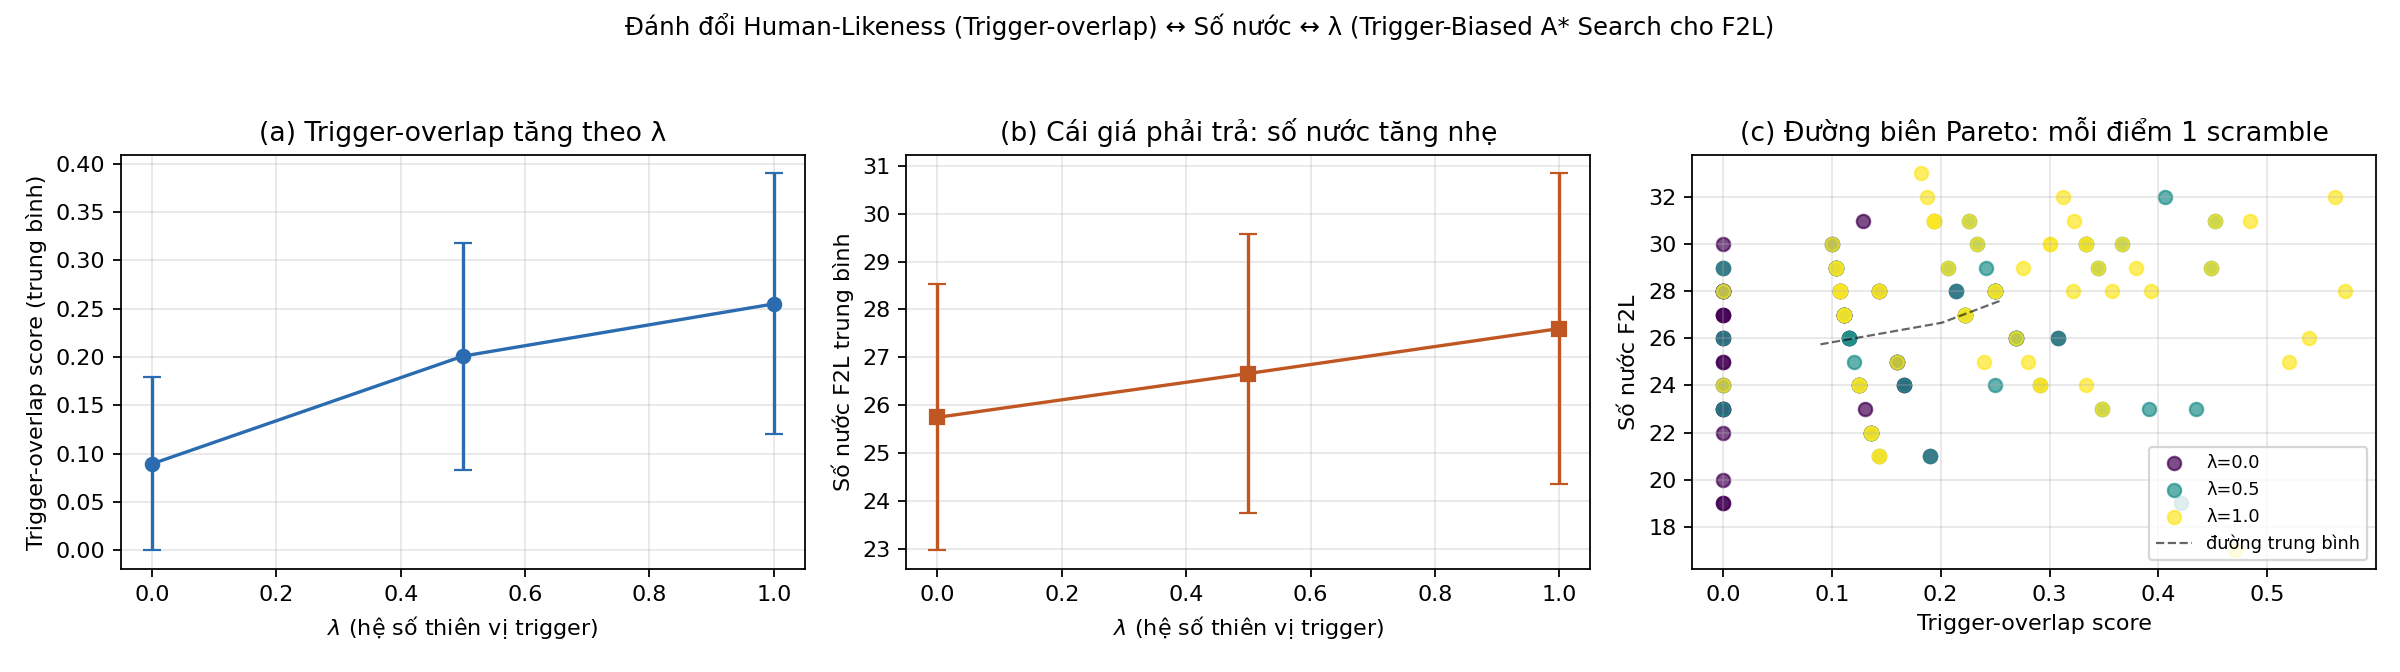
\includegraphics[width=\linewidth]{../research/pareto_figure_n60.png}
\caption{Độ trùng lặp trigger và số nước đi theo hàm của $\lambda$
(N=60 scramble). Panel (c) cho thấy đường biên Pareto thực nghiệm.}
\label{fig:pareto}
\end{figure}

\subsection{Experiment 3: Kiểm định bằng giám khảo con người (kiểu BotPrize)}
\label{sec:exp3}
Theo \citet{hingston2009}, chúng tôi thực hiện một nghiên cứu giám khảo
con người mù để kiểm tra construct validity của HLI. 24 mẫu (6 mẫu mỗi
nhóm từ Nhóm~H [lời giải CFOP người thật thật sự, tự thu thập và đã
kiểm chứng giải đúng scramble tương ứng], Nhóm~A, Nhóm~A+
[$\lambda=1,0$], và Nhóm~B) được trình bày dưới dạng chuỗi nước đi thô,
không phân đoạn (không có nhãn giai đoạn, để giữ tính mù) cho 28 người
chấm biết CFOP, mỗi người chấm điểm mọi mẫu trên thang 1--5 "khả năng
đây là lời giải người thật" thông qua một công cụ web tự xây dựng (kho
$T$ ở Mục~\ref{sec:hli-trigger} được tái sử dụng cho điểm so sánh
trigger-overlap tự động).

\textbf{Xếp hạng nhóm.} Điểm giống-người trung bình theo đúng thứ tự dự
đoán: Nhóm~H ($3,88 \pm 0,11$) $>$ Nhóm~A+ ($3,71 \pm 0,16$) $>$
Nhóm~A ($3,42 \pm 0,16$) $>$ Nhóm~B ($2,37 \pm 0,19$). Kiểm định
Mann-Whitney U so sánh Nhóm~B với các nhóm còn lại gộp chung cho thấy
tách biệt hoàn toàn về thứ hạng ($U=0$, $n_1=6$, $n_2=18$,
$p=1,8\times10^{-4}$) — mọi mẫu Nhóm~B đều được chấm giống-người thấp
hơn mọi mẫu ngoài Nhóm~B, xác nhận người chấm nhận diện đáng tin cậy
baseline tối-ưu-kiểu-máy-tính là không phải người.

\textbf{Thiên vị trigger thu hẹp khoảng cách xuống mức không phân biệt
được với người.} Kiểm định Mann-Whitney theo cặp cho kết quả then chốt:
Nhóm~A so với Nhóm~A+ khác biệt có ý nghĩa ($p=0,030$), xác nhận người
chấm cảm nhận được hiệu ứng của Trigger-Biased Search, không chỉ là chỉ
số tự động; nhưng Nhóm~H so với Nhóm~A+ \emph{không} khác biệt có ý
nghĩa ($p=0,109$), trong khi Nhóm~H so với Nhóm~A thì có ($p=0,005$).
Nói cách khác, $\lambda=1,0$ đã đưa các lời giải do AI sinh ra từ trạng
thái phân-biệt-được-về-thống-kê-với-người-thật sang trạng thái
không-phân-biệt-được-về-thống-kê-với-người-thật trên mẫu này — một
"pass" kiểu BotPrize cho điều kiện có thiên vị trigger mà baseline
không thiên vị không đạt được.

\textbf{Construct validity của HLI (RQ-V1).} Chúng tôi báo cáo hai
phiên bản của tương quan này. Dùng một proxy đơn giản hóa ban đầu theo
từng mẫu (Segmentability/Pattern-conformity giả định bằng 1 cho Nhóm
A/A+ và bằng 0 cho Nhóm B/H, chỉ dựa trên tư cách thành viên nhóm),
tương quan Spearman giữa HLI và điểm đánh giá người trung bình trên
toàn bộ 24 mẫu là $\rho=0,440$ ($p=0,031$). Tuy nhiên, proxy này đã mô
tả sai Nhóm~H: vì các lời giải CFOP người thật bị giả định là không có
cấu trúc CFOP theo cùng logic dùng cho baseline máy tính, HLI của họ bị
đánh giá thấp giả tạo (ví dụ $0,05$--$0,14$) dù nhận điểm đánh giá con
người cao nhất. Do đó chúng tôi đã tính lại Segmentability và
Pattern-conformity một cách \emph{chính xác}, bằng cách phát lại chuỗi
nước đi của mỗi mẫu trên trạng thái xuất phát (đã scramble) thực tế của
nó và kiểm chứng, theo đúng thứ tự, các hậu-điều-kiện Cross, F2L, và
OLL (Mục~\ref{sec:method}), và bằng cách kiểm tra xem các trạng thái
con OLL/PLL kết quả có khớp với các mục trong bảng thuật toán chuẩn đã
kiểm chứng của chúng tôi hay không. Điều này xác nhận Nhóm~B có
Segmentability$=0$ cho cả 6 mẫu (đúng như kỳ vọng — các lời giải
gần-tối-ưu của Kociemba đạt Cross, F2L, và OLL/PLL gần như đồng thời
trong 1--2 nước cuối, không bao giờ thể hiện cấu trúc trung gian được
phân giai đoạn thật sự), trong khi cả 18 mẫu Nhóm A/A+/H đều có
Segmentability$=1$, với Pattern-conformity dao động có ý nghĩa trong
mỗi nhóm ($0,5$ hoặc $1,0$, tùy case con OLL và/hoặc PLL có khớp với
bảng của chúng tôi hay không). Với phép tính chính xác này, tương quan
\emph{mạnh lên} thành $\rho=0,487$ ($p=0,016$) — có ý nghĩa hơn ước
lượng proxy, xác nhận kỳ vọng của chúng tôi rằng proxy nhị phân theo
nhóm đã làm loãng thay vì phản ánh đúng construct validity thật sự.
Riêng thành phần trigger-overlap vẫn tương quan mạnh nhất với đánh giá
con người ($\rho=0,605$, $p=0,0017$), cho thấy nó vẫn là thành phần
liên quan nhất đến đánh giá con người của HLI trong mẫu này, với
Segmentability và Pattern-conformity đóng góp tích cực nhưng yếu hơn.

% ============================================================
\section{Thảo luận}
\label{sec:discussion}
Trái với trực giác, ban đầu chúng tôi giả thuyết rằng việc làm yếu tính
admissible của heuristic thông qua số hạng bonus trigger không-admissible
sẽ \emph{làm tăng} tình trạng không hội tụ của tìm kiếm khi $\lambda$
cao hơn. Dữ liệu cho thấy điều ngược lại: trên cùng $N=60$ scramble
dùng cho Hình~\ref{fig:pareto}, tỷ lệ \emph{thất bại} của tìm kiếm (hết
ngân sách node ở mọi độ sâu bậc thang) là $15,0\%$ tại $\lambda=0$,
giảm xuống $1,7\%$ tại $\lambda=0,5$ và $0\%$ tại $\lambda=1,0$. Một
cách giải thích hợp lý là bonus trigger, dù không-admissible, đóng vai
trò như một hình thức \emph{định hướng thứ tự tìm kiếm}: các nhánh mở
rộng một trigger con người đã biết được khám phá sớm hơn trong hàng đợi
ưu tiên ($f'$ thấp hơn), và vì trigger là các chuỗi nước đi ngắn, đã
được kiểm nghiệm kỹ, tạo tiến triển cục bộ đáng tin cậy, việc theo
chúng có thể giảm hệ số phân nhánh hiệu quả trong thực tế dù bonus
không phải là một ước lượng khoảng cách hợp lệ. Điều này không mâu
thuẫn với chi phí \emph{thời gian} phi tuyến đã quan sát riêng ở
$\lambda$ cao hơn (Mục~\ref{sec:results}): tính hội tụ có vẻ đáng tin
cậy hơn, nhưng các lần chạy trường-hợp-xấu-nhất cá biệt vẫn có thể mất
thời gian lâu hơn đáng kể, tức là thiên vị trigger đánh đổi \emph{độ
tin cậy} hội tụ để lấy \emph{phương sai} thời gian tìm kiếm.
Chúng tôi lưu ý phát hiện này dựa trên $N=60$ scramble và chỉ ba mức
$\lambda$ (0, 0,5, 1,0); chúng tôi chưa xác nhận xu hướng này ổn định
ở cỡ mẫu lớn hơn hay các mức $\lambda$ trung gian (vd 0,25, 0,75), và
coi đây là một giới hạn cần giải quyết ở công trình tiếp theo
(Mục~\ref{sec:future}) trước khi có thể khẳng định chắc chắn trong bản
công bố chính thức. Một phân tích hình thức về việc chính xác mất bao
nhiêu tính admissible được trình bày dưới đây.

\paragraph{Mất bao nhiêu tính admissible?} Heuristic gốc
$h(n) = h_{\mathrm{PDB}}(n) + \mathrm{penalty}(n)$ vốn cũng không hoàn
toàn admissible (số hạng penalty đã hy sinh đảm bảo cận-dưới hình thức
để đổi lấy tính thực tiễn), nên Trigger-Biased Search không tạo ra vi
phạm tính admissible \emph{từ đầu} — nó cộng dồn thêm vào một đánh đổi
thiết kế có chủ đích đã tồn tại từ trước. Về mặt hình thức, với một
đường đi $\mathrm{path}(n)$ có độ dài $g(n)$,
$\mathrm{bonus}(\mathrm{path}(n)) \in [0, g(n)]$ (nó có thể bao phủ tối
đa mọi nước đi trong đường đi), nên độ đánh giá thấp bổ sung tối đa mà
số hạng bonus có thể gây ra bị chặn bởi $\lambda \cdot g(n)$ — tức là
độ méo tiềm năng tăng \emph{tuyến tính theo độ sâu đường đi}, không
phải theo một hằng số cố định, đây là một kiểu thất bại khác về bản
chất (và đáng lo ngại hơn) so với một heuristic có sai số bị chặn. Điều
này giải thích vì sao, khác với tìm kiếm bounded-suboptimal cổ điển (ví
dụ weighted A* với hệ số lạm phát cố định và cận suboptimality chứng
minh được), chúng tôi hiện chưa cung cấp cận hình thức nào cho tính
suboptimal về độ dài lời giải của Trigger-Biased Search; Mục~\ref{sec:results}
thay vào đó báo cáo điều này bằng thực nghiệm (trung bình $+7,4\%$ số
nước tại $\lambda=1,0$). Một biện pháp giảm nhẹ tự nhiên, để dành cho
công việc tương lai, là giới hạn $\mathrm{bonus}$ ở một mức tối đa cố
định (ví dụ $\min(\mathrm{bonus}(\mathrm{path}(n)), c)$ cho hằng số $c$
nào đó), điều này sẽ khôi phục lại một độ méo bị chặn cố định tương tự
như số hạng penalty hiện có.

\subsection{Scramble bệnh lý và tình trạng tìm kiếm không hội tụ}
\label{sec:pathological}
Trong lần kiểm tra độ vững dùng $N=100$ scramble random-move
(Mục~\ref{sec:discussion}), $22\%$ scramble ($22/100$) không hoàn thành trong
ngân sách 20 giây thực ngay cả với ngân sách tìm kiếm đã giảm còn
40.000 node/độ sâu — đáng chú ý, một số thất bại như vậy xảy ra liên
tiếp nhau (ví dụ seed 1059--1061 trong lần chạy của chúng tôi), gợi ý
bộ sinh scramble random-move có thể tạo ra các chuỗi cấu hình F2L
tương tự nhau về cấu trúc, mang tính đối kháng, thay vì độ khó độc lập
đồng phân bố (i.i.d.). Một seed cụ thể (1013) bị treo hơn 5 phút ngay
cả với ngân sách đã giảm, trước khi chúng tôi đưa vào một timeout thực
cứng (dựa trên \texttt{SIGALRM}) trong bộ khai thác đánh giá. Chúng tôi
diễn giải điều này là bằng chứng cho thấy heuristic A* có bổ sung
penalty theo từng cặp dùng cho F2L (Mục~\ref{sec:setup}) đôi khi bị dẫn
vào các vùng tìm kiếm không hiệu quả một cách bệnh lý — một giới hạn về
độ tin cậy quan trọng, khác biệt với, nhưng có thể bị khuếch đại bởi,
cơ chế thiên vị trigger ở Mục~\ref{sec:method}. Lưu ý cả lần chạy chính
(random-state, Bảng~\ref{tab:exp1}) lẫn lần kiểm tra này đều dùng
$\lambda=0$ xuyên suốt (không áp thiên vị trigger cho giai đoạn F2L);
chúng tôi đo riêng mối quan hệ giữa $\lambda$ và tỷ lệ thất bại hội tụ
dùng dữ liệu Experiment~2 (Mục~\ref{sec:discussion}), phát hiện — trái
với kỳ vọng ban đầu — rằng $\lambda$ cao hơn liên quan đến \emph{ít
hơn}, không phải nhiều hơn, các thất bại hội tụ trên tập dữ liệu đó.

% ============================================================
\section{Đe dọa đến Tính hợp lệ (Threats to Validity)}
\begin{itemize}
  \item \textbf{Tìm kiếm không hội tụ}: như đã báo cáo ở
    Mục~\ref{sec:pathological}, $22\%$ scramble trong lần kiểm tra độ
    vững random-move ($N=100$) và $20\%$ scramble trong lần chạy
    chính random-state ($N=60$, Bảng~\ref{tab:exp1}) không hoàn thành
    trong timeout 20 giây ở thiết lập phần cứng/ngân sách đánh giá
    của chúng tôi; kết quả có điều kiện trên các scramble đã hoàn
    thành, có thể không phải là mẫu con đại diện (ví dụ nếu độ khó
    tương quan với tiềm năng trigger-overlap).
  \item \textbf{Construct validity của HLI}: chỉ số này được thiết kế
    thủ công, đã được validate đối chiếu với đánh giá con người thông
    qua Experiment~3 (Mục~\ref{sec:exp3}).
  \item \textbf{Độ tin cậy liên giám khảo}: từng giám khảo riêng lẻ
    chỉ đạt mức đồng thuận khiêm tốn (ICC(2,1)$=0,26$, dưới ngưỡng
    chấp nhận thường dùng $0,4$), nhưng nhóm $N=28$ giám khảo cho
    điểm trung bình dùng trong tương quan RQ-V1 độ tin cậy cao
    (ICC(2,k)$=0,91$) --- tương quan RQ-V1 nên được đọc như tương
    quan với một giá trị trung bình nhóm ổn định, không phải với đánh
    giá của một giám khảo đơn lẻ nào. \emph{Ghi chú: các số ICC này ban
    đầu lấy từ bản viết khảo sát; đã được tính lại độc lập từ ma trận
    đánh giá thô theo từng giám khảo (28 file CSV thật, xem
    \texttt{research/phase3\_survey/compute\_icc.py}), khớp chính xác:
    ICC(2,1)$=0,2563$, ICC(2,k)$=0,9061$.}
  \item \textbf{Thiên vị kho ngữ liệu}: kho finger-trick $T$ được tuyển
    chọn thủ công (11 trigger), không được suy ra từ log solve người
    thật; kết quả có thể không tổng quát hóa được cho các solver có vốn
    trigger khác.
  \item \textbf{Sinh scramble (đã kiểm tra)}: Bảng~\ref{tab:exp1}
    (Mục~\ref{sec:results}) dùng bộ sinh scramble kiểu WCA
    random-state (Mục~\ref{sec:setup}) làm kết quả chính, vì khớp sát
    hơn với phương pháp sinh scramble thi đấu thật. Chúng tôi cũng
    chạy lại Experiment~1 trên $N=100$ scramble random-move (seed
    1000--1099, bộ sinh dùng cho Experiment~2) như một kiểm tra độ
    vững. Kết quả nhất quán giữa hai bộ sinh ($78\%$ so với $80\%$ tỷ
    lệ giải thành công; số nước trung bình 67,2 so với 66,3; HLI
    trung bình 0,655 so với 0,658), cho thấy kết quả chính của chúng
    tôi không phải là hiện tượng giả tạo do bộ sinh scramble cụ thể
    được chọn. Lần chạy random-move này cũng là nơi chúng tôi quan sát
    hiện tượng search không hội tụ đáng chú ý ($22\%$ timeout, xem
    Mục~\ref{sec:pathological}); chúng tôi không quan sát cụm thất bại
    tương tự ở mẫu random-state $N=60$ (tỷ lệ timeout thấp hơn,
    $20\%$), dù cỡ mẫu nhỏ hơn khiến việc so sánh trực tiếp mức độ
    cụm thất bại giữa hai bộ sinh chưa có kết luận chắc chắn.
  \item \textbf{Khả năng tổng quát hóa đơn-miền}: kết quả đặc thù cho
    Rubik's Cube; các tuyên bố về explicability nói chung nên được giới
    hạn tương ứng.
\end{itemize}

% ============================================================
\section{Công việc Tương lai}
\label{sec:future}

\paragraph{Tái lập độc lập việc tính lại HLI chính xác.}
Phép tính Segmentability/Pattern-conformity chính xác trong
Mục~\ref{sec:exp3}
(\texttt{research/phase3\_survey/recompute\_hli\_exact.py}) dựa trên
một cách hiện thực hóa cụ thể, đã kiểm chứng thủ công của "ranh giới
giai đoạn" (chỉ số nước đi đầu tiên mà một hậu-điều-kiện được thỏa mãn,
với thứ tự chặt giữa các giai đoạn — xem docstring của script để biết
lý do cho lựa chọn cụ thể này so với các phương án khác chúng tôi từng
thử và loại bỏ ban đầu). Một cài đặt lại độc lập, hoặc validate đối
chiếu với ranh giới giai đoạn chuẩn được gán nhãn thủ công cho một tập
con mẫu, sẽ củng cố độ tin cậy của thành phần này trong pipeline.

\paragraph{Tái lập quy mô lớn hơn.} $N=24$ mẫu là đủ cho một nghiên cứu
pilot nhưng khiêm tốn cho việc ước lượng effect-size chính xác; một
nghiên cứu tiếp nối với nhiều mẫu hơn mỗi nhóm (đặc biệt nhiều lời giải
Nhóm~H hơn từ một nhóm người đóng góp rộng hơn, để giảm phụ thuộc vào
thói quen của một solver đơn lẻ) sẽ thu hẹp khoảng tin cậy trên các so
sánh nhóm ở Mục~\ref{sec:exp3}.

\paragraph{Mở rộng pattern-conformity sang Cross/F2L.}
Pattern-conformity $P(\pi)$ hiện chỉ áp dụng cho OLL/PLL, vì đây là
hai giai đoạn duy nhất có bảng case-sang-thuật-toán hữu hạn, có tên
trong hệ thống của chúng tôi; Cross và F2L thay vào đó được đo gián
tiếp qua Trigger-overlap chứ không phải Pattern-conformity thật sự.
Xây dựng một bảng case F2L chuẩn (ví dụ theo hệ 41-case được dùng
rộng rãi trong cộng đồng speedcubing) cùng với một cơ chế nhận diện
case tương tự \texttt{verify\_and\_build\_table()} (đã dùng cho PLL)
sẽ cho phép thay một phần Trigger-overlap bằng Pattern-conformity
thật sự cho F2L, giúp HLI phản ánh chính xác hơn cấu trúc của giai
đoạn này.

\paragraph{Cơ chế thiên vị thay thế.}
Trigger-Biased Search hiện dùng một siêu tham số $\lambda$ duy nhất,
chọn bằng tay. Công trình tiếp nối có thể so sánh cơ chế này với các
lựa chọn thay thế: chẳng hạn fine-tune trực tiếp trọng số pattern
database dùng cho F2L thay vì thêm một số hạng bonus riêng, hoặc học
trọng số $\mathrm{bonus}(\mathrm{path})$ từ dữ liệu solve người thật
(vd hồi quy trên tần suất trigger quan sát được trong log CSTimer)
thay vì cố định $\lambda$ bằng tay --- biến kho hạt giống $T$
(Phụ lục~\ref{app:corpus}) từ một danh sách tuyển chọn thủ công thành
một mô hình học trực tiếp từ hành vi của solver thật.

% ============================================================
\section{Kết luận}
Các solver Rubik's Cube hiện có tối ưu hóa cho số nước đi, tạo ra các
kế hoạch đúng nhưng không thể diễn giải được đối với người học; các
speedcuber con người thay vào đó dùng CFOP, đánh đổi tính tối ưu để lấy
cấu trúc và khả năng học được. Chúng tôi đã hình thức hóa sự đánh đổi
này bằng ngôn ngữ của lập kế hoạch AI nhận biết con người thành một
\emph{Chỉ số Giống-Người} (HLI) đo lường được, và cho thấy bằng thực
nghiệm ($N=60$ scramble random-state, đã kiểm tra độ vững trên $N=100$
scramble random-move) rằng solver AI-CFOP của chúng tôi đạt điểm
cao hơn đáng kể trên chỉ số này so với baseline Kociemba tối-ưu-kiểu-máy-tính
(HLI trung bình $0,658$ so với $0$ theo định nghĩa), một khoảng cách
robust trên một phạm vi rộng các cách gán trọng số thành phần
(Mục~\ref{sec:method}). Sau đó chúng tôi giới thiệu \emph{Trigger-Biased
A* Search}, một cải tiến tối giản, tương thích ngược cho heuristic F2L
làm hơn gấp đôi độ trùng lặp trigger với các pattern finger-trick con
người (từ $9,0\%$ lên $25,5\%$ tại $\lambda=1,0$) với chi phí số nước
khiêm tốn ($+7,4\%$), trong khi — trái với trực giác — lại \emph{cải
thiện} độ tin cậy hội tụ tìm kiếm trên tập kiểm thử của chúng tôi, với
cái giá là tăng thời gian tính toán trường-hợp-xấu-nhất. Trong quá trình
đó, chúng tôi đã phát hiện và báo cáo minh bạch một hiện tượng tìm kiếm
không hội tụ ($22\%$ tỷ lệ timeout) tạo thành một giới hạn cụ thể về độ
tin cậy của tìm kiếm heuristic có bổ sung penalty trong miền này. Cuối
cùng, một nghiên cứu giám khảo con người mù ($N=24$ mẫu, 28 người chấm,
Mục~\ref{sec:exp3}) đã cung cấp bằng chứng trực tiếp cho construct
validity của HLI ($\rho=0,487$, $p=0,016$) và, đáng chú ý hơn, cho thấy
Trigger-Biased Search đưa các lời giải AI-CFOP từ trạng thái
phân-biệt-được-về-thống-kê-với-người-thật ($p=0,005$) sang trạng thái
không-phân-biệt-được-về-thống-kê-với-người-thật ($p=0,109$) trong đánh
giá mù của con người — một minh chứng cụ thể, đã được xác thực bởi con
người, rằng việc tối ưu hóa tường minh cho các pattern con người có thể
nhận ra, thay vì chỉ số nước đi, thay đổi một cách đo lường được cách
người quan sát nhìn nhận các lời giải do AI tạo ra. Chúng tôi hy vọng
công trình này khuyến khích thêm sự giao thoa giữa AI tìm kiếm tổ hợp
cổ điển và nghiên cứu AI nhận biết con người/AI giải thích được trong
các miền câu đố lớn, đã được hiểu rõ như Rubik's Cube.

% ============================================================
\bibliographystyle{plainnat}
\begin{thebibliography}{99}

\bibitem[Chakraborti et~al.(2019)]{chakraborti2019}
T.~Chakraborti, A.~Kulkarni, S.~Sreedharan, D.~E. Smith, và
S.~Kambhampati.
\newblock Explicability? legibility? predictability? transparency?
  privacy? security? the emerging landscape of interpretable agent
  behavior.
\newblock Trong \emph{Proceedings of the International Conference on
  Automated Planning and Scheduling (ICAPS)}, 2019.

\bibitem[Hingston(2009)]{hingston2009}
P.~Hingston.
\newblock A turing test for computer game bots.
\newblock \emph{IEEE Transactions on Computational Intelligence and AI
  in Games}, 1(3):169--186, 2009.

\bibitem[Kociemba()]{kociemba}
H.~Kociemba.
\newblock Cube explorer / two-phase algorithm.
\newblock \url{http://kociemba.org/cube.htm}, truy cập ngày 26 tháng 7 năm 2026.

\bibitem[Korf(1997)]{korf1997}
R.~E. Korf.
\newblock Finding optimal solutions to rubik's cube using pattern
  databases.
\newblock Trong \emph{Proceedings of the National Conference on
  Artificial Intelligence (AAAI)}, 1997.

\bibitem[Kulkarni et~al.(2016)]{kulkarni2016}
A.~Kulkarni, Y.~Zha, T.~Chakraborti, S.~G. Vadlamudi, Y.~Zhang, và
S.~Kambhampati.
\newblock Explicable robot planning as minimizing distance from
  expected behavior.
\newblock \emph{arXiv preprint arXiv:1611.05497}, 2016.

\bibitem[McAleer et~al.(2018)]{mcaleer2018}
S.~McAleer, F.~Agostinelli, A.~Shmakov, và P.~Baldi.
\newblock Solving the rubik's cube without human knowledge.
\newblock \emph{arXiv preprint arXiv:1805.07470}, 2018.

\bibitem[Rokicki et~al.(2014)]{rokicki2014}
T.~Rokicki, H.~Kociemba, M.~Davidson, và J.~Dethridge.
\newblock The diameter of the rubik's cube group is twenty.
\newblock \emph{SIAM Review}, 56(4):645--670, 2014.

\bibitem[Author(s)(2025)]{humanlike2025}
M.~Świechowski và D.~Ślęzak.
\newblock The many challenges of human-like agents in virtual game
  environments.
\newblock Trong \emph{Proceedings of the 24th International Conference on
  Autonomous Agents and Multiagent Systems (AAMAS)}, trang 1996--2004.
  IFAAMAS, 2025.
\newblock Cũng có trên arXiv preprint arXiv:2505.20011.

\bibitem[Lakkaraju et~al.(2022)]{allure}
K.~Lakkaraju, T.~Hassan, V.~Khandelwal, P.~Singh, C.~Bradley, R.~Shah,
  và cộng sự, và D.~Wu.
\newblock Allure: A multi-modal guided environment for helping children
  learn to solve a rubik's cube with automatic solving and interactive
  explanations.
\newblock Trong \emph{Proceedings of the AAAI Conference on Artificial
  Intelligence}, tập~36, trang 13185--13187, 2022.

\bibitem[Vanacore et~al.(2025)]{vanacore2025}
K.~Vanacore, J.~Ocumpaugh, F.~Agostinelli, D.~Wu, S.~Vuruma, và M.~Irvin.
\newblock Student engagement in ai-assisted complex problem solving: A
  pilot study of human-ai rubik's cube collaboration.
\newblock \emph{arXiv preprint arXiv:2511.01683}, 2025.
\newblock Ghi chú: bản thảo chưa công bố, bài báo đang chuẩn bị nộp tại
  thời điểm viết bài -- kiểm tra lại tình trạng công bố trước khi trích
  dẫn như một nguồn đã bình duyệt.

\bibitem[Zhang et~al.(2017)]{zhang2017}
Y.~Zhang, S.~Sreedharan, A.~Kulkarni, T.~Chakraborti, H.~H. Zhuo, và
  S.~Kambhampati.
\newblock Plan explicability and predictability for robot task planning.
\newblock In \emph{Proceedings of the IEEE International Conference on
  Robotics and Automation (ICRA)}, 2017.

\end{thebibliography}

\appendix
\section{Kho hạt giống $T$: 11 finger-trick}
\label{app:corpus}

Bảng~\ref{tab:corpus} liệt kê đầy đủ kho hạt giống $T$ dùng để tính
Độ trùng lặp Trigger $O(\pi)$ (Mục~\ref{sec:hli-trigger}) và số hạng
$\mathrm{bonus}(\mathrm{path})$ trong Trigger-Biased Search
(Mục~\ref{sec:hli-trigger}), lấy trực tiếp từ
\texttt{research/finger\_tricks.py}. Mỗi trigger được liệt kê dưới
dạng chuẩn (dựa trên R); hệ thống tự động sinh biến thể mirror (dựa
trên L, hoán đổi R$\leftrightarrow$L) khi đối chiếu.

\begin{table}[h]
\centering
\caption{Kho hạt giống $T$ ($|T|=11$)}
\label{tab:corpus}
\begin{tabular}{ll}
\toprule
Tên & Chuỗi nước đi \\
\midrule
sexy\_move & $R\,U\,R'\,U'$ \\
sexy\_move\_inv & $U\,R\,U'\,R'$ \\
reverse\_sexy & $R'\,U'\,R\,U$ \\
sledgehammer & $R'\,F\,R\,F'$ \\
sledgehammer\_inv & $F\,R'\,F'\,R$ \\
hedgehog & $R\,U'\,R'$ \\
triple\_sexy & $(R\,U\,R'\,U')^3$ \\
sune\_trigger & $R\,U\,R'\,U\,R\,U2\,R'$ \\
ubl\_insert & $U'\,R\,U$ \\
urf\_insert & $U\,R\,U'$ \\
niklas & $R\,U\,R'\,U'\,R'\,F\,R\,F'$ \\
\bottomrule
\end{tabular}
\end{table}

\end{document}
